
In cryptography, we are of course not just interested in abstract structure of Elliptic Curves and isogenies, but also in computing with them.
A fundamental algorithm based on the Velu formulas allows to compute the curve $E/G$ and the isogeny $E \to E/G$ for a finite subgroup $G \leq E$ in time polynomial in $\#G$.
However, in the general case, there is no way how one can represent or compute an isogeny of exponentially large degree.
This is where one can do cryptography, since for smooth-degree isogenies $\psi$, we can factor them into a sequence of small degree isogenies, and evaluate them one after the other.
However, if this factorization is not known, it seems very hard to evaluate the isogeny.

The underlying structure of this approach (and others) can now be captured by the $l$-isogeny graph $\Gamma_l(\F_q)$, for a prime $l \neq p$.
For this chapter, and the rest of this work, we assume $p = \mathrm{char}(k) \neq 2, 3$.
\begin{definition}
    Denote by $\Gamma_l(k)$ the graph whose vertices are isomorphism classes of Elliptic Curves over $k$, and the edges are the degree $l$ isogenies (again up to isomorphism
    \footnote{We say two isogenies $\phi, \psi: E \to E'$ are isomorphic, if there are automorphisms $\tau \in \mathrm{Aut}(E)$ and $\rho \in \mathrm{Aut}(E')$ such that $\phi = \rho \circ \psi \circ \tau$.
    Note that $\mathrm{Aut}(E) = \{ \pm 1 \}$ unless $j(E) \in \{ 0, 1728 \}$ (assuming $\mathrm{char}(k) \neq 2, 3$), so this case occurs only at the two vertices with j-invariants $0$ and $1728$.}) 
    between them (with multiplicity).
\end{definition}
Since there is never an isogeny between ordinary and supersingular curves, each connected component of $\Gamma_l(\F_q)$ contains either only ordinary or supersingular curves.
Hence, we will call them ordinary and supersingular connected components, respectively.
Furthermore, the existence of the dual isogeny shows that this graph is undirected.
We also know that if $p \neq 2, 3$ and $l \neq p$, the graph $\Gamma_l(\bar{\F}_p)$ is $(l + 1)$-regular except at the j-invariants $0$ and $1728$, since there are exactly $l + 1$ subgroups of order $l$ in $E[l] \cong (\Z/l\Z)^2$.

Note that when doing computations with this graph, we identify each vertex with the j-invariant of the corresponding curves.
This makes it easy to work with isomorphism classes of Elliptic Curves.
Furthermore, we observe that $\Gamma_l(\F_q)$ has exactly $q$ vertices, since there are that many j-invariants $j \in \F_q$.

\section{The ordinary case}
We begin by analyzing the structure of the ordinary part of $\Gamma_l(\F_q)$, which (as we will see), is quite different from the supersingular part.
There is a very powerful description of this graph in terms of the endomorphism rings of the ordinary curves.
Since these are (usually non-maximal) orders in quadratic imaginary number fields, whose theory is somewhat more complicated than the one of maximal orders (which are Dedekind domains), we first study them a little.

\subsection{Imaginary quadratic orders}
For this part, let $\O$ be an order in an imaginary quadratic number field $K$, and let $\O_K$ denote the maximal order in $K$.
What we will mainly do in this section is to show that ideal $\a \leq \O$ with norm $\Norm(\a) := [\O : \a]$ coprime to the index $[\O_K : \O]$ behave ``nicely'', i.e. similar to ideals in a Dedekind domain.
Furthermore, we will study the structure of the class group of $\O$.
First, we state a version of the Chinese remainder theorem.
\begin{lemma}
    Let $\a$ be a nonzero ideal of $\O$. Then
    \begin{equation*}
        \O/\a \cong \bigoplus_\p \O_\p/\a\O_\p
    \end{equation*}
\end{lemma}
For a proof of this, see e.g. \cite[Prop.~I.12.3]{neukirch}.
From now on, write $\Norm(\a)$ for the norm of an ideal $\a \leq \O$, i.e. $\Norm(\a) := [\O : \a]$.
In the Dedekind ring $\O_K$ this is multiplicative, in the order $\O$, it is (in general) not.
\begin{lemma}
    Let $\p \leq \O_K$ be a prime with $\Norm(\p) \perp [\O_K : \O]$.
    Then $\p$ has a set of generators in $\O$.
\end{lemma}
\begin{proof}
    Suppose $\p$ is a prime over $p$, and write $\O = \Z[\phi]$ for a generator $\phi$ of $\O$.
    We use the decomposition law in Dedekind ring extensions.
    Since $\Norm(\p) \perp [\O_K : \O]$ are coprime, we can apply it for the generator $\phi$ of $\O$.

    If $\mathrm{MiPo}(\phi) = f(X)g(X) \mod p$ splits, then have
    \begin{equation*}
        p\O_K = (p, f(\phi))(p, g(\phi))
    \end{equation*}
    and so the prime ideals over $p$ are $(p, f(\phi))$ and $(p, g(\phi))$.
    If $\mathrm{MiPo}(\phi) \mod p$ is irreducible, then have that $p\O_K$ is prime and thus the only prime ideal over $p$.
    Hence, all prime ideals over $p$ (including $\p$) have a set of generators in $\O$.
\end{proof}
Since multiplication of ideals can be expressed by the product of their generators, we get the following corollary.
\begin{corollary}
    \label{prop:generators_in_order}
    Let $\a \leq \O_K$ be an ideal with $\Norm(\a) \perp [\O_K : \O]$. Then $\a$ has a set of generators in $\O$.
\end{corollary}
\begin{prop}
    \label{prop:prime_coprime_localization_same}
    Let $\p \leq \O$ be a prime ideal with $\Norm(\p) \perp [\O_K : \O]$ and $\p' = \p\O_K$.
    Then $\O_\p = (\O_K)_{\p'}$.
\end{prop}
\begin{proof}
    We can choose a generator $\alpha$ of $\O_K$ and find $\O_K = \Z[\alpha]$ as well as $\O = \Z[f\alpha]$ where $f = [\O_K : \O]$.
    Thus $f \notin \p$ and so $f \in \O_\p^*$.
    Therefore $\alpha = f^{-1}f\alpha \in \O_\p$ and so $(\O_K)_{\p'} \subseteq \O_\p$.
\end{proof}
\begin{lemma}
    If $\a \leq \O$ with $\Norm(\a) \perp f := [\O_K : \O]$ then also $\Norm(\a\O_K) \perp f$.
    Conversely, if $\a \leq \O_K$ with $\Norm(\a) \perp f$, then also $\Norm(\a \cap \O) \perp f$.
\end{lemma}
\begin{proof}
    For the first statement, note that if $\Norm(\a) \perp f$, then also $\a \perp f\O$ and so there is a relation $1 = a + fb$ with $a \in \a$ and $b \in \O$.
    However, then $1 \in \a\O_K + f\O_K$ and so $\a\O_K \perp f$, thus $\Norm(\a\O_K) \perp f$.

    On the other hand, for $\a \leq \O_K$ with $\Norm(\a) \perp f$, we have the map
    \begin{equation*}
        \O \to \O_K/\a, \quad x \mapsto [x]
    \end{equation*}
    It clearly has kernel $\a \cap \O$, and so we find that $\O/(\a \cap \O) \subseteq \O_K/\a$.
    Thus $\Norm(\a \cap \O) \divides \Norm(\a)$ and it follows that $\Norm(\a \cap \O) \perp f$.
\end{proof}
Instead of all ideals in $\O$, we often only work with the set of invertible (fractional) ideals.
A fractional ideal $\a \leq \O$ is invertible, if there is another fractional ideal $\b$ with $\a\b = \O$.
In contrast to the set of all ideals, this is now a group.
Clearly, every ideal $\a$ of the Dedekind ring $\O_K$ is invertible.

This already gives a somewhat nice description of most ideals of the order $\O$.
\begin{prop}
    \label{prop:coprime_ideals_order}
    Let $\mathfrak{I}_f(\O)$ resp. $\mathfrak{I}_f(\O_K)$ denote the monoid of invertible integral ideals of norm $\perp f := [\O_K : \O]$.
    Then
    \begin{align*}
        \mathfrak{I}_f(\O) \to \mathfrak{I}_f(\O_K), \quad \a \mapsto \a\O_K
    \end{align*}
    is a monoid isomorphism with inverse
    \begin{equation*}
        \mathfrak{I}_f(\O_K) \to \mathfrak{I}_f(\O), \quad \a \mapsto \a \cap \O
    \end{equation*}
\end{prop}
\begin{proof}
    Clearly, this is a well-defined monoid homomorphism.
    Hence, we have to show that it is bijective.

    By Corollary~\ref{prop:generators_in_order}, we know that any $\a \leq \O_K$ with $\Norm(\a) \perp [\O_K : \O]$ has generators in $\O$, thus $(\a \cap \O)\O_K = \a$.
    This shows that $\a \cap \O$ is a preimage of $\a$, and so the map is surjective. 

    Assume now $\a, \b \leq \O$ with $\a\O_K = \b\O_K$ and $\Norm(\a), \Norm(\b) \perp f$.
    We show that $\a\O_\p = \b\O_\p$ for all primes $\p \leq \O$.
    Note that if $\Norm(\p) \not\perp f$, this holds trivially, as $\a\O_\p = \O_\p = \b\O_\p$.
    Otherwise, note that
    \begin{equation*}
        \a\O_\p = \a (\O_K)_\p = \a\O_K(\O_K)_\p = \b\O_K(\O_K)_\p = \b (\O_K)_\p = \b\O_\p
    \end{equation*}
    as $\O_\p = (\O_K)_\p$.
    This shows that $\a\O_\p = \b\O_\p$ at all primes, so $\a = \b$ and our map is injective.
    Furthermore, since $(\a \cap \O)\O_K = \a$, we see that it has the inverse
    \begin{equation*}
        \mathfrak{I}_f(\O_K) \to \mathfrak{I}_f(\O), \quad \a \mapsto \a \cap \O
    \end{equation*}
    which must then be well-defined.
\end{proof}
Furthermore, we are interested in the class group of $\O$, which is now the quotient of only the invertible ideals of $\O$ modulo the principal ideals.
The following statements are special cases of the general theory in \cite[Chapter I.§12]{neukirch}.
\begin{lemma}
    \label{prop:invertible_ideal_characterization}
    Write $\mathfrak{I}(\O)$ for the group of invertible fractional ideals in $\O$.
    Then there exists an isomorphism
    \begin{equation*}
        \iota: \bigoplus_\p K^*/\O_\p^* \to \mathfrak{I}(\O)
    \end{equation*}
    with $\iota(a)\O_\p = (a_\p)$ for all prime ideals $\p \leq \O$ and $a = (a_\p)_\p$.
\end{lemma}
\begin{proof}
    This proof is taken with some modifications from \cite[Prop.~I.12.9]{neukirch}.

    First, we show that for an invertible ideal $\a = (a_1, ..., a_n)$ have that $\a\O_\p$ is principal.
    By assumption, have $\a\b = (1)$ with $\b = (b_1, ..., b_m)$ and so have $1 = \sum a_i b_i c_i$ with $c_i \in \O$.
    Clearly, $1 \notin \p\O_\p$ and thus one $a_i b_i c_i \notin \p\O_\p$, so $a_i b_i c_i \in \O_\p^*$ is a unit.
    Therefore, we find that $\a\O_\p = a_i\O_\p$, because for all $x \in \a\O_\p$, have then $x b_i c_i \in \a\b = \O_\p$, so
    \begin{equation*}
        x = a_i \underbrace{x b_i c_i}_{\in \O_\p} (\underbrace{a_ib_ic_i}_{\in\O_\p^*})^{-1} \in a_i \O_\p
    \end{equation*}
    Now we can see that there is a well-defined homomorphism
    \begin{equation*}
        \iota^{-1}: \mathfrak{I}(\O) \to \bigoplus_\p K^*/\O_\p^*
    \end{equation*}
    that maps an ideal $\a$ to the class of generators of $\a\O_\p$.
    
    Clearly, it is injective, since if $\a\O_\p \neq \b\O_\p$ for any prime $\p$, then $\a \neq \b$.

    It is thus left to show that $\iota^{-1}$ is also surjective.
    The following proof is taken with some modifications from \cite[Prop.~I.12.2]{neukirch}.

    Let $(a_\p)_\p \in \bigoplus_\p K^*/\O_\p^*$ and set $\a := \bigcap_\p a_\p \O_\p$.
    We claim that $\iota^{-1}(\a) = (a_\p)_\p$. 
    Clearly we have $\a\O_\p \subseteq a_\p\O_\p$, so it is left to show the inclusion $\supseteq$.

    By multiplying both $(a_\q)_\q$ and $\a$ with an appropriate constant, we can assume that all $a_\q \in \O$.
    Furthermore, all but finitely many $a_\q \in \O_\q^*$, so assume wlog those are $a_\q = 1$.

    Let $b \in \O \setminus \{ 0 \}$ with $ba_\q/a_\p \in \O$ for all finitely many $\q$, $a_\q \neq 1$.

    Now the Chinese remainder theorem gives us $c \in \O$ such that
    \begin{equation*}
        c \equiv b \mod \p \quad \text{and} \quad c \equiv b a_q/a_\p \mod \q^k \quad \text{for $\q \neq \p$, $a_\q \neq 1$}
    \end{equation*}
    where $k \geq 1$ is an integer such that $\q^k\O_\q \subseteq a_\q\O_\q$.
    Technically, $c$ is only unique modulo $\p \cap \bigcap_{\q \neq \p, a_\q \neq 1} \q$, but we are satisfied with any representative.

    Now note that $c/b \in \O_\p^*$.
    Therefore, we can choose $d \in \O \setminus \p$ with $dc/b \in \O$.
    Hence, also $\epsilon := dc/b \in \O_\p^*$ and $\epsilon \in \O$.
    We claim that $a_\p \epsilon \in \a$ and the claim follows.

    We have
    \begin{itemize}
        \item $a_\p \epsilon \in a_\p\O_\p$ since $\epsilon \in \O \subseteq \O_\p$.
        \item $a_\p \epsilon \in a_\q\O_\q$ for $\q \neq \p$, $a_\q \neq 1$ since $a_\p c/b \equiv a_\q \mod \q^k$, thus $a_\p c/b \in a_\q\O_\q$ and finally $a_\p \epsilon = d a_\p c/b \in a_\q\O_\q$.
        \item $a_\p \epsilon \in a_\q\O_\q$ for $\q$ with $a_\q = 1$, since $a_\p, \epsilon \in \O$, thus $a_\p \epsilon \in \O \subseteq \O_\q = a_\q\O_\q$.
    \end{itemize}
    The claim follows.
\end{proof}
This lemma is a very useful characterization of invertible ideals.
We are now ready for our first description of $\Cl(\O)$.
\begin{lemma}
    Let $f = [\O_K : \O]$ and assume that $\O_K^* = \{ \pm 1 \}$.
    There is an exact sequence
    \begin{equation*}
        1 \ \to \ \bigoplus_\p R_\p^*/\O_\p^* \overset{f}{\longrightarrow} \Cl(\O) \overset{g}{\longrightarrow} \Cl(\O_K) \ \to \ 1
    \end{equation*}
    where $\Cl(\O)$ is the ideal class group of $\O$, i.e. the group of invertible, fractional ideals modulo principal ideals and $R_\p$ is the localization of $\O_K$ at the multiplicative set $\O \setminus \p$.
\end{lemma}
\begin{proof}
    This proof is taken with some modifications from \cite[Prop.~I.12.11]{neukirch}.

    First, we show that every ideal class $[\a] \in \Cl(\O_K)$ has an integral representative of norm coprime to $f$.
    Let $m \divides \Norm(\a)$ be maximal such that $m \divides f^e$ for some $e$.
    Then there is an element $\alpha \in m\a^{-1}$, and we see that $\Norm(\alpha^{-1}\a) \divides \Norm(\a)/m$, thus is coprime to $f$.
    Furthermore, $\alpha \in \a^{-1}$, so $\alpha^{-1}\a$ is integral.
    This shows our claim, and so by Corollary~\ref{prop:generators_in_order} that the natural map
    \begin{equation*}
        \Cl(\O) \to \Cl(\O_K), \quad [\a] \to [\a\O_K]
    \end{equation*}
    is surjective.

    Next, note that the isomorphism $\iota: \bigoplus_\p K^*/\O_\p^* \to \mathfrak{I}(\O)$ induces a map
    \begin{equation*}
        \bigoplus_\p R_\p^*/\O_\p^* \to \Cl(\O)
    \end{equation*}
    where $R_\p$ is the localization of $\O_K$ at the multiplicative subset $\O \setminus \p$.

    It is injective, as for an element $a = (a_\p)_\p$ in the kernel, have that $\iota(a) = (\alpha)$.
    However, then $(a_\p) = (\alpha)$ in $\O_\p$.
    Hence, $a_\p = \alpha\epsilon$ for $\epsilon \in \O_\p^*$ and we can assume that the representatives $a_\p \in R_\p^*$ are chosen such that $a_\p = \alpha$.
    This implies that $\alpha \in \O \cap \bigcap_\p R_\p^* = \O_K^*$, and by the assumption $\O_K^* = \{ \pm 1 \}$, have then $\alpha = \pm 1$.
    The claim follows.

    Now it is only left to show that the sequence is exact at $\Cl(\O)$.

    For $a = (a_\p)_\p \in \bigoplus_\p R_\p^*/\O_\p^*$, we know that
    \begin{equation*}
        \iota(a)R_\p = \iota(a)\O_\p R_\p = a_\p R_\p = R_\p
    \end{equation*}
    and so $\mathrm{im}(f) \subseteq \ker(g)$.
    Now we show the converse.

    Let $\a \leq \O$ be integral and invertible with $\a\O_K = (\alpha)$.
    Since $[\frac 1 \alpha \a] = [\a]$ are in the same ideal class, we can assume wlog that $\alpha = 1$.

    Let $a = (a_\p)_\p = \iota^{-1}(\a)$.
    Then
    \begin{equation*}
        a_\p R_\p = a_\p\O_\p R_\p = \iota(a)R_\p = \a R_\p = \alpha R_\p = R_\p
    \end{equation*}
    This clearly implies that $a_\p \in R_\p^*$ and so $\a \in \mathrm{im}(f)$.
\end{proof}
The expression $\bigoplus_\p R_\p^*/\O_\p^*$ is still somewhat unwieldy, but fortunately, it has the following nice form.
\begin{lemma}
    We have
    \begin{equation*}
        (\O_K/f\O_K)^*/(\O/f\O_K)^* \cong \bigoplus_\p R_\p^*/\O_\p^*
    \end{equation*}
    Note that $f\O_K \subseteq \O$ is the largest ideal of $\O_K$ contained in $\O$, and thus an ideal of $\O$ as well.
\end{lemma}
\begin{proof}
    First, note that if $\Norm(\p) \perp f$, we know that $R_\p = (\O_K)_{\p\O_K}$ and so by Prop.~\ref{prop:prime_coprime_localization_same} that $R_\p^*/\O_\p^*$ is trivial.
    
    Note that for each prime $\p \leq \O$ containing $f\O_K$ have a finite, positive number of primes $\q \leq \O_K$ with $\q \cap \O = \p$.
    There is at least one, as $\p\O_K$ is contained in a prime, and the number is finite, as $f\O_K$ factors into finitely many primes in the Dedekind ring $\O_K$.
    Hence, we have by the Chinese remainder theorem
    \begin{equation*}
        (\O/f\O_K)^* \cong \bigoplus_{\p \supseteq f\O_K} (\O_\p/f\O_K\O_\p)^* = \bigoplus_{\p \supseteq f\O_K} (\O_\p/fR_\p)^*
    \end{equation*}
    Furthermore, we have
    \begin{equation*}
        (\O_K/f\O_K)^* \cong \bigoplus_{\q \supseteq f\O_K} ((\O_K)_\q/f(\O_K)_\q)^* \cong \bigoplus_{\p \supseteq f\O_K} \bigoplus_{\q \supseteq \p\O_K} ((\O_K)_\q/f(\O_K)_\q)^*
    \end{equation*}
    We claim that
    \begin{equation*}
        R_\p/fR_\p \cong \bigoplus_{\q \supseteq \p\O_K} (R_\p)_\q/f(R_\p)_\q = \bigoplus_{\q \supseteq \p\O_K} (\O_K)_\q/f(\O_K)_\q
    \end{equation*}
    This isomorphism follows from the Chinese remainder theorem and the fact that the prime ideals $\q$ over $\p\O_K$ give all prime ideals of $R_\p$.
    
    Both isomorphisms are compatible
    \footnote{Meaning the inclusion $\O/f\O_K \subseteq \O_K/f\O_K$ commutes with the natural map
    \begin{equation*}
        O/f\O_K \overset{\sim}{\to} \bigoplus_\p (\O_\p/f\O_K\O_\p) = \bigoplus_\p (\O_\p/fR_\p) \to \bigoplus_\p (R_\p/fR_\p) \overset{\sim}{\to} \O_K/f\O_K
    \end{equation*}
    }, 
    and so have
    \begin{equation*}
        (\O_K/f\O_K)^*/(\O/f\O_K)^* \cong \bigoplus_{\p \supseteq f\O_K} (R_\p/fR_\p)^*/(\O_\p/fR_\p)^*
    \end{equation*}
    Finally, observe that the map $R_\p^* \to (R_\p/fR_\p)^*/(\O_\p/fR_\p)^*$ has kernel $\O_\p^*$.
    It also is surjective, since for $[a] \in (R_\p/fR_\p)^*$ there is $b \in R_\p$ with $ab \in 1 + fR_\p$ and thus $ab \equiv 1 \mod \p R_\p$ (because we only consider $\p$ with $f \in \p$).
    In particular, $a \notin \q$ for all primes $\q$ of $R_\p$ (these are all over $\p R_\p$), and so $a \in R_\p^*$.
\end{proof}
\begin{corollary}
    \label{prop:class_group_order}
    Suppose $\O_K = \{ \pm 1 \}$. Then there is an exact sequence
    \begin{equation*}
        1 \ \to \ (\O_K/f\O_K)^*/(\O/f\O_K)^* \ \to \ \Cl(\O) \ \to \ \Cl(\O_K) \ \to \ 1
    \end{equation*}
\end{corollary}
The condition $\O_K = \{ \pm 1 \}$ is very weak, as there are only two quadratic imaginary number fields such that the ring of integers has more units, namely $K = \Q[\sqrt{-3}]$ and $K = \Q[\sqrt{-1}]$.
These correspond to the Elliptic Curves with j-invariants $0$ and $1728$ (if they are ordinary), and need a special treatment in many cases anyway.
In \cite{neukirch}, there is also a more general version of this statement without this assumption.

\subsection{The class group action}
Now we can come back to the study of Elliptic Curves and their isogeny graphs.
The class group action which we will define in the following is the most important tool when working with isogeny graphs of ordinary curves.
Because of this, it is mentioned in more or less all the literature dealing with the topic.
For me, it was thus quite surprising that I could nowhere find a precise and relatively elementary proof for the statement in the case of finite fields.

Most sources cite \cite[Thm~4.5]{class_group_action_waterhouse}, however the statement there is not as explicit as one might wish, and the proof is done in the much more general theory of abelian schemes.
Apart from that, there are many references to the corresponding statement for curves over $\C$, but these ignore some of the subtleties introduced by non-separable isogenies. 
Therefore, we now present a relatively simple proof of the class group action for ordinary curves defined over a finite field and explicitly handle the non-separable case.

For the whole section, let $E$ and $E'$ be Elliptic Curves defined over a finite field $k = \F_q$ with characteristic $p$.
We write $\pi_E$ for the $q$-th power Frobenius endomorphism of $E$.
\begin{definition}
    For an integral ideal $\a \leq \End(E)$ of an ordinary Elliptic Curve $E$, define the $\a$-torsion
    \begin{equation*}
        E[\a] := \bigcap_{\alpha \in \a} \ker(\alpha)
    \end{equation*}
\end{definition}
From now on, we will often compare endomorphism rings of isogenous curves.
To do so, we embed those rings into an imaginary quadratic number field $K$.
However, the field $K$ and its orders can have nontrivial automorphisms, which means the embedding $\End(E) \to K$ cannot be unique.
Fortunately, we can choose a system of embeddings $\End(E) \to K$ jointly for all curves $E$ in a canonical way as follows.
\begin{lemma}
    Let $\phi: E \to E'$ be an isogeny.
    Then there is an isomorphism
    \begin{equation*}
        \Phi: \End(E) \otimes \Q \to \End(E') \otimes \Q, \quad \tau \mapsto \frac 1 {\deg(\phi)} \phi \circ \tau \circ \hat{\phi}
    \end{equation*}
    Furthermore, if we assume $E$ to be ordinary, then this is canonical in the sense that for any other isogeny $\psi: E \to E'$ have $\Phi = \Psi$.
\end{lemma}
\begin{proof}
    It is clear that this is a morphism of ring, and its inverse is given by $\hat{\Phi}$ induced by the dual isogeny $\hat{\phi}$.
    
    So it remains to show the last part.
    Let $\phi$ and $\psi$ be two isogenies $E \to E'$.
    Then for each $\tau \in \End(E)$ have
    \begin{align*}
        (\Phi \circ \hat{\Psi})(\tau) =& \frac 1 { \deg(\phi) } \phi \circ \left( \frac 1 {\deg(\psi)} \hat{\psi} \circ \tau \circ \psi \right) \circ \hat{\phi} \\
        =& \frac 1 { \deg(\phi)\deg(\psi) } (\phi \circ \hat{\psi}) \circ \tau \circ (\psi \circ \hat{\phi}) \\
        =& \frac 1 { \deg(\phi)\deg(\psi) } (\phi \circ \hat{\psi}) \circ (\psi \circ \hat{\phi}) \circ \tau \\
        =& \frac 1 { \deg(\phi)\deg(\psi) } (\deg(\phi) \deg(\psi)) \tau = \tau
    \end{align*}
    since $(\psi \circ \hat{\phi})$ and $\tau$ are elements of $\End(E)$, hence commute.

    Now $\hat{\Psi}$ is the inverse of $\Psi$, and the claim follows.
\end{proof}
In other words, we choose an arbitrary embedding $\End(E) \to K$ for one ordinary curve $E$, and then choose all further embeddings $\End(E') \to K$ for isogenous curves $E'$ as
\begin{equation*}
    \End(E') \to \End(E') \otimes \Q \ \overset{\Phi}{\longrightarrow} \ \End(E) \otimes \Q \to K
\end{equation*}
From now on, whenever we identify $\End(E)$ with an appropriate subring of $K$, this shall use that embedding.
It will already be used in the next statement, which describes the relationship of endomorphism rings of isogenous curves more concretely.
\begin{prop}
    Let $\phi: E \to E'$ be an isogeny of prime degree $p$ between ordinary Elliptic Curves.
    Then (after embedding $\End(E')$ via $\Phi$ and $\End(E)$ into $\End(E) \otimes \Q$) exactly one of the following is the case.
    \begin{itemize}
        \item $\End(E) = \End(E')$ and we call $\phi$ \emph{horizontal}.
        \item $\End(E) \subseteq \End(E')$ with $[\End(E') : \End(E)] = p$. We call $\phi$ \emph{ascending}.
        \item $\End(E) \supseteq \End(E')$ with $[\End(E) : \End(E')] = p$. We call $\phi$ \emph{descending}.
    \end{itemize}
\end{prop}
\begin{proof}
    Note that the map
    \begin{equation*}
        p\Phi: \End(E) \to \End(E'), \quad \tau \mapsto \phi \circ \tau \circ \hat{\phi}
    \end{equation*}
    yields endomorphisms of $\End(E')$, and so we have $p\End(E) \subseteq \End(E')$.
    Similarly, find $p\End(E') \subseteq \End(E)$.

    Now let $\alpha$ be a generator of the maximal order in $K = \End(E) \otimes \Q$.
    Then each order of $K$ is of the form $\Z \oplus f\alpha\Z$, and so
    \begin{equation*}
        \End(E) = \Z \oplus f_1\alpha\Z, \quad \End(E') \Z \oplus f_2\alpha\Z
    \end{equation*}
    However, this implies that $f_1 \divides pf_2$ and $f_2 \divides pf_1$, so $f_1 \divides p f_2 \divides p^2 f_1$.
    Since $p$ is prime, we find $f_2 \in \{ f_1/p, f_1, p f_1 \}$ and the claim follows.
\end{proof}
Furthermore, we will sometimes talk about horizontal or vertical isogenies \emph{at a prime $l$}, which is defined by the next proposition.
The advantage is that this is defined for all isogenies, not just those of prime degree.
\begin{prop}
    Similarly, let $\phi: E \to E'$ be an isogeny of any degree $n$.
    Further, let $l$ be a prime.
    Then (after embedding $\End(E') \otimes \Z_{(l)}$ via $\Phi$ and $\End(E) \otimes \Z_{(l)}$ into $\End(E) \otimes \Q$) exactly one of the following is the case.
    \begin{itemize}
        \item $\End(E) \otimes \Z_{(l)} = \End(E') \otimes \Z_{(l)}$ and we call $\phi$ \emph{horizontal at $l$}.
        \item $\End(E) \otimes \Z_{(l)} \subseteq \End(E') \otimes \Z_{(l)}$ with $[\End(E') \otimes \Z_{(l)} : \End(E) \otimes \Z_{(l)}] = l^r$ for $r > 0$. We call $\phi$ \emph{ascending at $l$}.
        \item $\End(E) \otimes \Z_{(l)} \supseteq \End(E') \otimes \Z_{(l)}$ with $[\End(E) \otimes \Z_{(l)} : \End(E') \otimes \Z_{(l)}] = l^r$ for $r > 0$. We call $\phi$ \emph{descending at $l$}.
    \end{itemize}
\end{prop}
\begin{proof}
    Exactly as the previous proof.
\end{proof}
Now we can make a step towards the class group action and present how we assign isogenies to (integral, invertible) ideals of the endomorphism ring.
\begin{definition}
    For an ordinary Elliptic Curve $E$ and an integral, invertible ideal
    \footnote{By Prop.~\ref{prop:coprime_ideals_order}, this representation of an ideal $\a$ is well-defined and unique, as $\Norm((p, \pi)) = p \notdivides [\O_{\End(E) \otimes \Q} : \End(E)] \divides d(\End(E))$.}
    $\a = \b(p, \pi_E)^r \leq \End(E)$ with $\b \perp (p, \pi_E)$ define the isogeny
    \begin{equation*}
        \phi_{E, \a}: E \ \longrightarrow \ E/E[\b] \ \overset{\pi_r}{\longrightarrow} \ E_\a := (E/E[\b])^{(p^r)}
    \end{equation*}
    where $E \to E/E[\b]$ is the unique separable isogeny with kernel $E[\b]$ and $\pi_r: E/E[\b] \to (E/E[\b])^{(p^r)}$ is the $r$-th power Frobenius map.
\end{definition}
In order to define a group action later, we need to be able to chain such isogenies given by ideals.
The obvious difficulty here is that the ideals are all in the same ring, but subsequent isogenies will have different curves as domain.
Hence, we need to be able to view an ideal $\a \leq \End(E)$ as an ideal of another endomorphism ring $\End(E')$.
As it turns out, the endomorphism rings we consider are all isomorphic, and so this works out nicely. 
\begin{lemma}
    Let $E$ be an ordinary Elliptic Curve and $\a \leq \End(E)$ an integral, invertible ideal.
    Then $\End(E) \cong \End(E_\a)$.
    In particular, $\phi_{E, \a}$ is horizontal at every prime $l$.
\end{lemma}
\begin{proof}
    Let $\a = \b(p, \pi_E)^r$ with $\b \perp (p, \pi_E)$.
    We show that $\End(E) \cong \End(E/E[\b])$ and the claim follows, as for any Elliptic Curve $E$, have an isomorphism
    \begin{equation*}
        \End(E) \to \End(E^{(p)}), \quad \alpha \mapsto \alpha^{(p)}
    \end{equation*}
    It suffices to show that the separable isogeny $\phi := \phi_{E, \b}$ is horizontal at each prime $l$.

    Assume for a contradiction that $\phi$ is descending at $l$.
    In other words, there is $\tau \in \End(E)$ such that $\phi \circ \tau \circ \hat{\phi}$ is not divisible by $l$.
    Hence, $E'[l] \not\subseteq \ker(\phi \circ \tau \circ \hat{\phi})$ and there is a point $P \in E'[l]$ with $\phi(\tau(\hat{\phi}(P))) \neq \IdPoint$.
    This implies $\tau(\hat{\phi}(P)) \notin E[\b]$ and thus there is $\alpha \in \b$ with $\tau(\hat{\phi}(P)) \notin \ker(\alpha)$.
    Note that $\alpha$ factors through $\phi$ as
    \begin{center}
        \begin{tikzpicture}
            \node (Ep) at (0, 0) {$E'$};
            \node (E1) at (-4, 0) {$E$};
            \node (E2) at (4, 0) {$E$};

            \draw [->] (E1) -- (Ep) node [midway, above] {$\phi$};
            \draw [->] (Ep) -- (E2) node [midway, above] {$\psi$};
            \draw [->] (E1) to [bend left] node [midway, above] {$\alpha$} (E2);
        \end{tikzpicture}
    \end{center}
    We assume $l \divides \deg(\phi)$, otherwise the claim is trivial.
    However, then we have the contradiction
    \begin{align*}
        \IdPoint \neq \psi((\phi \circ \tau \circ \hat{\phi})(P)) &= (\psi \circ \phi \circ \tau \circ \hat{\phi})(P) = (\alpha \circ \tau \circ \hat{\phi})(P) \\
        &= (\tau \circ \alpha \circ \hat{\phi})(P) = (\tau \circ \psi \circ [n])(P) = (\tau \circ \psi)(\IdPoint) = \IdPoint
    \end{align*}
    since $\tau \circ \alpha = \alpha \circ \tau$ ($\End(E)$ is commutative).
\end{proof}
For the next statement, we need to establish the relationship between separability of endomorphisms and properties of the endomorphism ring.
\begin{lemma}
    \label{prop:inseparable_iff_frobenius_ideal}
    Let $E$ be an ordinary curve and $\alpha \in \End(E)$.
    Then $\alpha$ inseparable if and only if $\alpha \in (p, \pi_E)$.
\end{lemma}
\begin{proof}
    First, consider
    \begin{equation*}
        \b := \{ \beta \in \End(E) \ | \ \text{$\beta$ inseparable} \}
    \end{equation*}
    This is an ideal, as for two inseparable $\beta_1, \beta_2 \in \End(E)$ have that they factor as
    \begin{center}
        \begin{tikzpicture}
            \node (Ep) at (0, 0) {$E^{(p)}$};
            \node (E1) at (-4, 0) {$E$};
            \node (E2) at (4, 0) {$E$};

            \draw [->] (E1) -- (Ep) node [midway, above] {$\pi_1$};
            \draw [->] (Ep) -- (E2) node [midway, above] {$\phi_i$};
            \draw [->] (E1) to [bend left] node [midway, above] {$\beta_i$} (E2);
        \end{tikzpicture}
    \end{center}
    with the $p$-th power Frobenius $\pi_1: E \to E^{(p)}$.
    Now $\beta_1 + \beta_2 = (\phi_1 + \phi_2) \circ \pi_1$ is inseparable, and clearly $\beta \gamma$ is inseparable for $\beta \in \b$ and $\gamma \in \End(E)$ (just compare separability degrees).

    Furthermore, $p$ and $\pi_E$ are inseparable, so $(p, \pi) \subseteq \b$.
    Note that in the imaginary quadratic order $\End(E)$, every prime ideal is maximal.
    Since $\Norm((p, \pi)) = p \perp d(\End(E))$, Prop.~\ref{prop:coprime_ideals_order} shows that $(p, \pi_E)$ is prime, and thus $(p, \pi_E) = \b$ (clearly, $\b \neq \End(E)$).
\end{proof}
Note now that for an isogeny $\phi: E \to E'$, have
\begin{equation*}
    \phi \circ \hat{\phi} \circ \Phi(\pi_E) = \frac {\deg(\phi)} {\deg(\phi)} \phi \circ \pi_E \circ \hat{\phi}
\end{equation*}
Comparing inseparability degrees, it follows that $\Phi(\pi_E)$ is totally inseparable as endomorphism on $E'$.
Hence, $E'$ is isomorphic to a curve such that $\Phi(\pi_E)$ becomes the Frobenius endomorphism of that curve.
Since we only work with isomorphism classes, we assume from now on that $\Phi(\pi_E)$ is the Frobenius of $E'$.

Now we can prove that ideal multiplication is compatible with chaining of isogenies.
Note that the condition $p \notdivides d(\O)$ is just equivalent to all curves $E$ with $\End(E) \cong \O$ being ordinary.
\begin{lemma}
    Let $\O$ be a quadratic imaginary order with $p \notdivides d(\O)$ and two integral, invertible ideals $\a, \b \leq \O$.
    Let further $E$ be an Elliptic Curve with $\End(E) \cong \O$.
    Identifying $\End(E_\a)$ with $\O$ by the canonical isomorphism $\Phi_{E, \a}: \End(E) \overset{\sim}{\longrightarrow} \End(E_\a)$, we have
    \begin{equation*}
        E_{\a\b} \cong (E_\a)_\b \quad \text{and} \quad \phi_{E, \a\b} = \phi_{E_\a, \b} \circ \phi_{E, \a}
    \end{equation*}
\end{lemma}
\begin{proof}
    Write $\pi \in \O$ for the unique element of $\O$ that maps to the Frobenius of $E$ under the maps $\O \overset{\sim}{\longrightarrow} \End(E)$ for all $E$ with $\End(E) \cong \O$.
    
    We have $\a = \tilde{\a} (p, \pi)^r$ and $\b = \tilde{\b} (p, \pi)^s$ with $\tilde{\a}, \tilde{\b} \perp (p, \pi)$.
    For $q$ such that $\phi_{E_\a, \tilde{b}}$ is defined over $\F_q$, it is now the case that
    \begin{equation*}
        \phi_{E, \a\b} = \pi_{r + s} \circ \phi_{E, \tilde{\a} \tilde{\b}}
    \end{equation*}
    and
    \begin{equation*}
        \phi_{E_\a, \b} \circ \phi_{E, \a} = \pi_s \circ (\phi_{E_\a, \tilde{\b}} \circ \pi_r \circ \phi_{E, \tilde{\a}}) = \pi_{r + s} \circ (\phi_{E_\a, \tilde{\b}}^{(q/p^r)} \circ \phi_{E, \tilde{\a}})
    \end{equation*}
    where $\pi_r: E_{\tilde{\a}} \to E_{\tilde{\a}}^{(p^r)}$ is the $p^r$-th power Frobenius, and similar for $\pi_s$, $\pi_{r + s}$. 
    Note that $\phi_{E_\a, \tilde{\b}}$ is the separable isogeny with kernel $E_\a[\tilde{\b}]$ and thus $\phi_{E_\a, \tilde{\b}}^{(q/p^r)}$ is the separable isogeny with kernel $E_{\a}^{(q/p^r)}[\tilde{\b}] = E_{\tilde{\a}}[\tilde{\b}]$.
    In other words, find
    \begin{equation*}
        \phi_{E_\a, \tilde{\b}}^{(q/p^r)} = \phi_{E_{\tilde{\a}}, \tilde{\b}}
    \end{equation*}
    and so it suffices to show the claim in the case that $\a = \tilde{\a}$, $\b = \tilde{\b}$ are integral, invertible ideals coprime to $(p, \pi)$.
    By Lemma~\ref{prop:inseparable_iff_frobenius_ideal}, this means that the isogenies $\phi_{E, \a}$ and $\phi_{E_\a, \b}$ are separable.

    Having reduced everything to the separable case, it now suffices to show that $\ker(\phi_{E_\a, \b} \circ \phi_{E, \a}) = E[\a\b]$.
    For simplicity of notation, write $\phi = \phi_{E, \a}$ and $\psi = \phi_{E_\a, \b}$.
    Hence, we want to show that $\ker(\psi \circ \phi) = E[\a\b]$.

    The crucial point here is that our isomorphism $\End(E) \cong \End(E_\a)$ is given by $\Phi$.
    Since the identification of $\End(E)$ and $\End(E_\a)$ would hide this, we will be explicit in this part and write
    \begin{align*}
        i: \O \overset{\sim}{\longrightarrow} \End(E) \quad \text{and} \quad i': \O \overset{\sim}{\longrightarrow} \End(E')
    \end{align*}
    for the isomorphisms.
    Note that $\Phi \circ i = i'$.
    We have
    \begin{align*}
        \ker(\psi \circ \phi) =& \phi^{-1}(\ker\psi) = \phi^{-1}(E'[\mathfrak{a}]) = \phi^{-1}\Bigl( \bigcap_{\tau \in \mathfrak{a}} \ker(i'(\tau)) \Bigr) \\
        =& \bigcap_{\tau \in \mathfrak{a}} \phi^{-1}(\ker(i'(\tau))) = \bigcap_{\tau \in \mathfrak{a}} \ker(i'(\tau) \circ \phi) \overset{(*)}{=} \bigcap_{\tau \in \mathfrak{a}} \ker(\phi \circ i(\tau)) \\
        =& \bigcap_{\tau \in \mathfrak{a}} i(\tau)^{-1}(\ker\phi) = \bigcap_{\tau \in \mathfrak{a}} i(\tau)^{-1}(E[\mathfrak{b}]) = \bigcap_{\tau \in \mathfrak{a}, \ \rho \in \mathfrak{b}} i(\tau)^{-1}(\ker(i(\rho))) \\
        =& \bigcap_{\tau \in \mathfrak{a}, \ \rho \in \mathfrak{b}} \ker(\underbrace{i(\rho) \circ i(\tau)}_{\mathclap{= i(\rho\tau) \in i(\a\b)}}) = E[\mathfrak{b}\mathfrak{a}]
    \end{align*}
    The equality at $(*)$ holds, since
    \begin{equation*}
        i'(\tau) = (\Phi \circ i)(\tau) = \frac 1 {\deg(\phi)} \phi \circ i(\tau) \circ \hat{\phi} \qedhere
    \end{equation*}
\end{proof}
What we have so far is already enough to establish a monoid action
\begin{equation*}
    \mathfrak{I}(\O) \times \Ell(\O) \to \Ell(\O), \quad \a \mapsto E_{\a}
\end{equation*}
where $\mathfrak{I}(\O)$ stands for the monoid of integral invertible ideals of $\O$ and
\begin{equation*}
    \Ell(\O) := \{ \text{$E$ isomorphism class of Elliptic Curves over $\bar{\F}_p$} \ | \ \End(E) \cong \O \}
\end{equation*}
denote the set of isomorphism classes of Elliptic Curves with endomorphism ring $\O$.

Next, we investigate the torsion of this action, i.e. for which $\a$ we have $\a.E = E$.
\begin{lemma}
    Let $E$ be an ordinary curve and $\a, \b \leq \End(E)$ two integral, invertible ideals.
    Then $E_\a \cong E_\b$ if and only if $[\a] = [\b] \in \Cl(\End(E))$ are in the same ideal class.
\end{lemma}
\begin{proof}
    First, we show the direction $\Leftarrow$.
    By assumption, there are $\alpha, \beta \in \O$ such that $\alpha\a = \beta\b$.
    Thus $E_{\alpha\a} = E_{\beta\b}$ and it suffices to show that for any Elliptic Curve $E$ and $\alpha \in \End(E)$, have $E_{(\alpha)} \cong E$.

    Write $(\alpha) = (p, \pi)^r \a$ and assume that $E$ is defined over $\F_{p^s}$.
    It follows that $(p, \pi)^s = (\pi)$ and so there is $\alpha' \in \O$, $\alpha' \notin (p, \pi)$ with $(\alpha)(p)^{\lceil r/s \rceil s - r} = (\pi)^{\lceil r/s \rceil} (\alpha')$.
    Furthermore, $\alpha' \notin (p, \pi)$.
    Now note that for any curve $E$, have $E_{(\pi)} = E^{(p^s)} \cong E$ and $E_{(p)} \cong E$, where the latter holds, since in the ordinary case, $p$ factors as
    \begin{center}
        \begin{tikzpicture}
            \node (Ep) at (0, 0) {$E^{(p)}$};
            \node (E1) at (-4, 0) {$E$};
            \node (E2) at (4, 0) {$E$};

            \draw [->] (E1) -- (Ep) node [midway, above] {$\pi_1$};
            \draw [->] (Ep) -- (E2) node [midway, above] {$\phi$};
            \draw [->] (E1) to [bend left] node [midway, above] {$[p]$} (E2);
        \end{tikzpicture}
    \end{center}
    with the $p$-th power Frobenius $\pi_1$ and $\phi$ is separable with $\ker(\phi) = E[p] = \ker([p]) \cap \ker(\pi - t)$.
    Thus we see that $E_{(\alpha)} \cong E_{(\alpha')}$ and can assume wlog that $\alpha = \alpha' \notin (p, \pi)$.

    By Lemma~\ref{prop:inseparable_iff_frobenius_ideal}, we now see that $\alpha$ is separable, and so clearly $\ker(\alpha) = E[(\alpha)]$.
    Since $\alpha: E \to E$ is the separable isogeny on $E$ with kernel $E[(\alpha)]$, we see that $E_{(\alpha)} = E/E[(\alpha)] \cong E$.

    Now we consider the other direction $\Rightarrow$.
    Again, write $\a = \tilde{\a}(p, \pi)^r$ and assume that $E$ is defined over $\F_{p^s}$.
    Then we have as before that $\a (p)^{\lceil r/s \rceil s - r} = (\pi)^{\lceil r/s \rceil} \a'$ for the ideal $\a' = \tilde{\a} (p, \pi - t)^{\lceil r/s \rceil s - r}$.
    Now clearly $[\a] = [\a']$ are in the same ideal class and $\a' \perp (p, \pi)$.
    Furthermore, by the direction $\Leftarrow$, have $E_\a \cong E_{\a'}$.
    Doing the same with $\b$, we can assume wlog that $\a = \a'$ and $\b = \b'$ are ideals coprime to $(p, \pi)$.

    Therefore, the isogenies $\phi_{E, \a}$ and $\phi_{E, \b}$ are separable.
    Write $E' := E_\a = E_\b$.
    Choose $N > 0$ such that $[N]^{-1}(E[\a]) \supseteq E[\b]$.
    Note that $[N] \circ \phi_{E, \a} = \phi_{E, \a} \circ [N]$ and so the isogeny $[N] \circ \phi_{E, \a}$ factors through $\phi_{E, \b}$, i.e. we get a commutative diagram
    \begin{center}
        \begin{tikzpicture}
            \node (E1) at (0, 1) {$E'$};
            \node (E2) at (0, -1) {$E'$};
            \node (E0) at (-4, 0) {$E$};
            \node (E3) at (4, 0) {$E'$};

            \draw [->] (E0) -- (E1) node [midway, above] {$\phi_{E, \a}$};
            \draw [->] (E0) -- (E2) node [midway, above] {$\phi_{E, \b}$};
            \draw [->] (E1) -- (E3) node [midway, above] {$[N]$};
            \draw [->] (E2) -- (E3) node [midway, above] {$\psi$};
        \end{tikzpicture}
    \end{center}
    for some endomorphism $\psi: E' \to E'$.
    Clearly the isogenies $[N]$ and $\psi$ are given by the ideals $(N)$ resp. $(\psi)$, and so we find
    \begin{equation*}
        E[(N)\a] = E[(\psi)\b]
    \end{equation*}
    and the claim follows.
\end{proof}
Now we have proven almost everything we need.
The final ingredient, from which it will then follow that the class group action is transitive, is a theorem of Tate.
Since it uses much theory on general abelian varieties, we will present it without proof here.
For a proof, the reader is referred to the work of Tate \cite{tate}.
\begin{theorem}[Isogeny theorem]
    \label{prop:isogeny_theorem}
    Let $E$, $E'$ be Elliptic Curves defined over $\F_q$.
    Then there is an isogeny $E \to E'$ if and only if $\#E(\F_q) = \#E'(\F_q)$.
\end{theorem}
Note that this condition is also equivalent to $\End(E) \otimes \Q \cong \End(E') \otimes \Q$ or that the $q$-th power Frobenius endomorphisms have the same trace. 
\begin{theorem}
    \label{prop:class_group_action}
    Let $\O$ be an imaginary quadratic order with $p \notdivides d(\O)$.
    Then there is a free and transitive group action
    \begin{equation*}
        \Cl(\O) \times \Ell(\O) \to \Ell(\O), \quad ([\a], E) \mapsto E_\a
    \end{equation*}
    where $\a$ is an integral, invertible ideal representative of the ideal class $[\a]$.
\end{theorem}
\begin{proof}
    Well-definedness and freeness follow from all the previous lemmas.
    So it is left to derive the transitivity from Theorem~\ref{prop:isogeny_theorem}.
    Let $E$ and $E'$ be curves in $\Ell(\O)$.
    Clearly, we then have $\#E(\F_q) = \#E'(\F_q)$ and so there is an isogeny $\phi: E \to E'$.
    Everything we have to show is that $\phi = \phi_{E, \a}$ for some ideal $\a \leq \O$.
    Note that we can multiply $\a$ by $(p)$ and divide by $\pi$, and thus achieve that $\phi$ is separable.

    Here we use the same approach as in \cite[Thm~4.5]{class_group_action_waterhouse}.
    In particular, we want to consider the problem locally at primes $l$.
    The usual way to achieve this is to consider the $l$-adic Tate module defined as the inverse limit
    \begin{equation*}
        T_lE := \lim_n E[l^n]
    \end{equation*}
    Furthermore, the isogeny $\phi$ induces a map
    \begin{equation*}
        \phi_l: T_lE \to T_lE', \quad (P_n)_n \mapsto (\phi P_n)_n
    \end{equation*}
    An endomorphism $\alpha$ of $E$ now acts on $T_lE$, and so $T_lE$ becomes a free $\O_l := (\O \otimes \Z_l)$-module of rank 1.
    Also $T_lE'$ becomes an $\O_l$-module (this is where we use the assumption that $\End(E) \cong \End(E')$).
    Additionally, our choice of the canonical isomorphism $\End(E) \cong \O \cong \End(E')$ implies that $\phi_l$ is an $\O_l$-module homomorphism.
    Extending it linearly, we get the map
    \begin{equation*}
        \phi_l: T_lE \otimes_{\Z_l} \Q_l \to T_lE' \otimes_{\Z_l} \Q_l
    \end{equation*}
    We can now consider the $\O_l$-module $M := \phi_l^{-1}(T_lE') \subseteq T_lE \otimes_{\Z_l} \Q_l$.

    The module $M$ contains $T_lE$ and furthermore, $T_lE$ has finite index in $M$.
    Therefore $M$ is a $\O_l$-submodule of $l^{-n}T_lE$ for some $n$.

    So we see that $M$ is a free rank-1 module over $\O_l$, and hence there is an element $\alpha_l \in \O_l$ with
    \begin{equation*}
        \alpha_l M = T_lE
    \end{equation*}
    Note that we can write $\alpha_l = a \otimes l^n b$ with $a \in \O$ and $b \in \Z_l^*$.
    Then also $(al^n) M = T_lE$ and thus we can assume wlog that $\alpha_l = al^n \in \O$.

    Now it is left to establish the connection between $\ker(\phi)$ and $M$.
    This is done by the map
    \begin{equation*}
        \phi_l^{-1}(T_lE') = M \to \ker(\phi)_{(l)}, \quad \frac 1 {l^m} (P_n)_n \mapsto P_m
    \end{equation*}
    where an element of $T_lE'$ is $(P_n)_n$ with $P_n \in E[l^n]$ such that $[l]P_{n + 1} = P_n$.
    Further
    \begin{equation*}
        \ker(\phi)_{(l)} := \{ P \in \ker(\phi) \ | \ \text{$[l]^nP = \IdPoint$ for some $n \geq 0$}\}
    \end{equation*}
    is the power-of-$l$ torsion part of $\ker(\phi)$, or equivalently the localization at the prime ideal $(l)$ as $\Z$-module.

    First, note that the map is well-defined, as for an element $1/l^m (P_n)_n$ in the domain, we have by assumption
    \begin{equation*}
        \frac 1 {l^m} \phi_l((P_n)_n) = \frac 1 {l^m} (\phi(P_n))_n \in T_lE'
    \end{equation*}
    and thus $\phi(P_m) = \IdPoint$, i.e. $P_m \in \ker(\phi)$.

    Clearly, the map is also a morphism of $\O$-modules, where $\ker(\phi)_{(l)}$ becomes an $\O$-module in the obvious way.
    
    It is also surjective, since for $P \in \ker(\phi)_{(l)}$ of order $\mathrm{ord}(P) = l^m$, we can lift it to an element $(P_n)_n$ with $P_m = P$.
    Then clearly $1/l^m(P_n)_n \in M$ with image $P$.

    Finally, note that for $1/l^m(P_n)_n \in M$ have $P_m = \IdPoint$ if and only if $P_0 = ... = P_m = \IdPoint$, in which case we have that
    \begin{equation*}
        1/l^m(P_n)_n = (P_{n + m})_n \in T_lE
    \end{equation*}
    Thus the kernel of above map is $T_lE$ and we get an isomorphism of $\O$-modules
    \begin{equation*}
        \ker(\phi)_{(l)} \cong M / T_lE
    \end{equation*}

    Now let $\a \leq \O$ be the invertible ideal such that $\a\O_\l = (\alpha_l)_\l$ for every prime ideal $\l$ under a prime number $l$ (the $\alpha_l$ are the element from above with $\alpha_l M = T_lE$).
    This is possible by Lemma~\ref{prop:invertible_ideal_characterization}, as only finitely many $(\alpha_l) \neq (1)$ (namely those $l$ with $l \divides \deg(\phi)$).

    Then for each primes $l$, we have
    \begin{equation*}
        \ker(\phi)_{(l)} = \{ P \in E_{(l)} \ | \ \alpha_l(P) = \IdPoint \} = \{ P \in E_{(l)} \ | \ \forall \alpha \in \a: \alpha(P) = \IdPoint \}
    \end{equation*}
    where again $E_{(l)}$ is the power-of-$l$ torsion part of the group $E$.
    Thus $\ker(\phi) = E[\a]$.
\end{proof}
A similar class group action exists in many other cases, since it is really founded in the theory of abelian varieties, see \cite{class_group_action_waterhouse}.
Notable examples are the CSIDH class group action for supersingular curves defined over $\F_p$ (see \cite{csidh}), its generalization to so-called oriented curves (see \cite{osidh}), and the very classical class group action of Elliptic Curves with complex multiplication (over $\C$).
More concretely, if we consider an order $\O$ in a quadratic imaginary number field and write $\Ell(\O)$ for the set of (isomorphism classes of) curves over $\C$ with endomorphism ring $\O$ (these are said to have \emph{complex multiplication}), then there is a free and transitive class group action
\begin{equation*}
    \Cl(\O) \times \Ell(\O) \to \Ell(\O), \quad ([\a], E) \to E/E[\a]
\end{equation*}
where we choose $\a$ to be an integral ideal representative of $[\a]$.
Note that for ideals $\a \perp (p, \pi)$, this is analogous to our action defined above.
However, since the Frobenius has trivial kernel, one needs some addition in the finite field case.

Note that one can still keep the simpler definition
\begin{equation*}
    \Cl(\O) \times \Ell(\O) \to \Ell(\O), \quad ([\a], E) \to E/E[\a]
\end{equation*}
also in the finite field case, if we require $\a$ to be an (integral) ideal representative of $[\a]$ that is coprime to $(p, \pi)$.
Clearly, every ideal class has such a representative, since we can multiply with the principal ideal $(p) = (p, \pi)(p, \pi - t)$ and divide out the principal ideal $(\pi) = (p, \pi)^s$.
However, some sources do not explicitly mention that $\a$ must be chosen coprime to $(p, \pi)$, which caused me some confusion at the beginning.

\subsection{Volcanoes}
Once we have the class group action, we can derive a lot of information about the structure of the ordinary part of an isogeny graph.
\begin{definition}
    For $l > 0, d \geq 0$, a graph $G$ is called \emph{$l$-volcano of depth $d$}, if its vertices can be partitioned into a set $C$ (the ``crater'') and a set $L$ (the ``lava flows'') such that
    \begin{itemize}
        \item $G[C]$ is either a single vertex (possibly with one or two loops), two connected vertices or a cycle of at least two vertices\footnote{A cycle of two vertices shall be two vertices with a double edge.}
        \item $G[V]$ is a forest of complete $l$-ary trees of depth $d$
        \item Every vertex $v \in C$ is connected to the roots of $l + 1 - \deg_{G[C]}(v)$ trees in $G[L]$
    \end{itemize}
    In particular, every vertex in $G$ except the leaves of the trees has degree $l + 1$.
\end{definition}
The term ``volcano'' was introduced by \cite{isogeny_vulcano}, after Kohel had mostly determined the structure of ordinary connected components in his PhD thesis.
\begin{theorem}
    \label{prop:isogeny_vulcano}
    Let $G$ be a connected component of $\Gamma_l(\F_q)$.
    Suppose that $G$ is ordinary, i.e. its vertices are (isomorphism classes of) ordinary curves.
    Then $G$ is an $l$-volcano.
    Further, we have
    \begin{itemize}
        \item All curves on the crater have the same endomorphism ring $\O$ with $l \notdivides [\O_{\O \otimes \Q} : \O]$.
        \item All curves on the $i$-th tree level of a lava flow have the endomorphism ring $\Z + l^i\O$.
        \item The size of the crater is the order of $\l_1$ in $\Cl(\O)$, where $(l) = \l_1\l_2$ in $\O$, or 1 if $l$ is inert.
    \end{itemize} 
\end{theorem}
\begin{proof}
    This follows from the class group action and the description of the class group of quadratic imaginary orders (Corollary~\ref{prop:class_group_order}).
    For the remaining details, we refer the reader to Kohel's thesis \cite[Prop.~23]{kohel}.
\end{proof}
We remark that the crater of a volcano is a single vertex with a loop, if $(l)$ is inert in $\O$.
Furthermore, the crater consists of two connected vertices, if $(l)$ is ramified in $\O$, and is either a vertex with double loop or a cycle, if $(l)$ splits.
\begin{figure}
    \begin{minipage}{0.5\textwidth}
        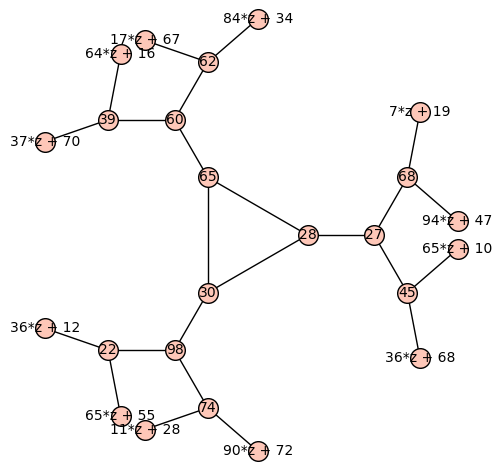
\includegraphics[width = \textwidth]{../example_odd_crater_fp.png}
    \end{minipage}%
    \begin{minipage}{0.5\textwidth}
        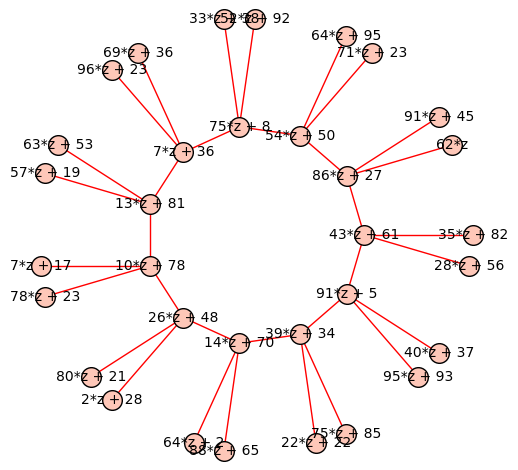
\includegraphics[width = \textwidth]{../example_odd_crater.png}
    \end{minipage}
    \begin{minipage}{0.5\textwidth}
        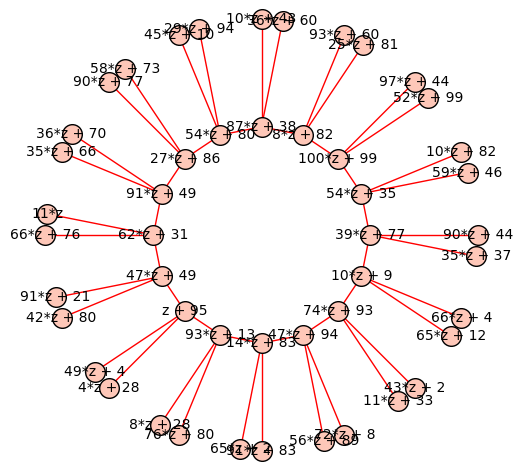
\includegraphics[width = \textwidth]{../example_II.png}
    \end{minipage}%
    \begin{minipage}{0.5\textwidth}
        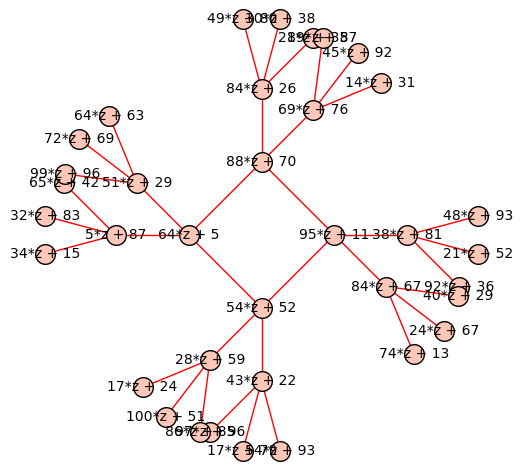
\includegraphics[width = \textwidth]{../example_III.png}
    \end{minipage}
    \caption{
        \label{fig:example_vulcanos} Examples of different 2-and 3-isogeny volcanoes in $\F_{101^2}$. 
        The value $\mathrm{z}$ is the generator of $\F_{101^2}$ with minimal polynomial $x^2 + 97x + 2$.
    }
\end{figure}

\section{The supersingular case}
\label{sec:supersingular_isogeny_graph}
After studying the ordinary connected components of the $l$-isogeny graph $\Gamma_l(\F_q)$, we now come to the supersingular component(s).
First, note that all supersingular j-invariants are defined over $\F_{p^2}$, and so we will assume $q = p^2$ for this section.

In the supersingular setting, the endomorphism ring is now non-commutative.
There still exists a non-commutative analogue of the class group action, but using it is significantly harder.
Mainly, because the theory of quaternion algebras is more complicated, and its class group structure is less studied.
\begin{figure}
    \begin{center}
        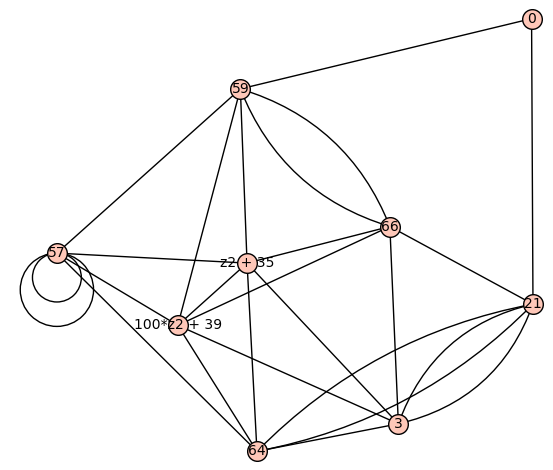
\includegraphics[width = 0.5\textwidth]{../example_supersingular.png}
    \end{center}
    \caption{
        \label{fig:example_supersingular_graph} The supersingular 3-isogeny graph over $\F_{101^2}$.
        The element $\mathrm{z}$ is a generator of $\F_{101^2}$ as in Figure~\ref{fig:example_vulcanos}.
    }
\end{figure}
Instead, there is the famous result of Pizer, which states that supersingular isogeny graphs (i.e. the supersingular part of $\Gamma_l(\F_q)$) are so called Ramajuan graphs, that is have excellent expander properties.
We will introduce this result in this section, but without proof.
\begin{definition}
    \label{def:expander}
    A $d$-regular graph $G$ is called $\epsilon$-expander, if the eigenvalues $\lambda_1 > ... > \lambda_n$ of its adjacency matrix satisfy
    \begin{equation*}
        |\lambda_2|, |\lambda_n| \leq (1 - \epsilon) d
    \end{equation*}
\end{definition}
In the literature, expander graphs are often defined by the use of the expansion ration
\begin{equation*}
    h(G) := \min_{S \subseteq V, \ \#S \leq \frac n 2} \frac {\#\partial S} {\# S}
\end{equation*}
of a graph $G = (V, E)$.
Here $\partial S$ is the edge boundary, i.e. the set of edges between a point in $S$ and a point in $V \setminus S$.

The connection between those two definitions is then given by the Cheeger-inequality
\begin{prop}
    Let $G$ be a $d$-regular graph such that its adjacency matrix has eigenvalues $\lambda_1 > ... > \lambda_n$.
    Then
    \begin{equation*}
        \frac {d - \lambda_2} 2 \leq h(G) \leq \sqrt{2d(d - \lambda_2)}
    \end{equation*}
\end{prop}
\begin{proof}
    See e.g. \cite{cheeger_inequality}.
\end{proof}
This inequality only correlates the so-called spectral gap $d - \lambda_2$ with $h(G)$, and does not bound $|\lambda_n|$.
In many cases, bounds on the spectral gap or expansion ration already suffice to show properties of expanders.
Because of this, expanders are usually defined as graphs for which only $\lambda_2$ or $h(G)$ are bounded.
Our definition~\ref{def:expander} is then sometimes called ``two-sided expander''.
However, we will never use one-sided expanders in this work, hence the above definition shall be sufficient.

The nice thing about the expansion ratio is that it gives more intuition on what the expander property means.
In particular, an expander graph is densely connected, i.e. by deleting a small number of edges, it is impossible to make the graph split into two (or more) connected components of relatively large size.
\begin{definition}
    A connected $d$-regular graph is called Ramajuan, if
    \begin{equation*}
        |\lambda_2|, |\lambda_n| \leq 2\sqrt{d - 1}
    \end{equation*}
    where $\lambda_1 > ... > \lambda_n$ are again the eigenvalues of the adjacency matrix.
\end{definition}
It is known that the bound $2\sqrt{d - 1}$ is asymptotically optimal, i.e. for sufficiently large $n$, all $d$-regular graphs of $n$ vertices have $\lambda_2 \geq 2\sqrt{d - 1} - \epsilon$.
In that sense, we can say Ramajuan graphs are graphs with asymptotically optimal expansion properties.

One of the main properties of expander graphs is that random walks on them mix rapidly.
That is, the final vertex of relatively short random walks is distributed almost uniformly among all vertices.
\begin{theorem}
    \label{prop:expander_random_walk}
    Let $G = (V, E)$ be a $d$-regular $\epsilon$-expander graph and $v \in V$ a vertex.
    Then the distribution of the final vertex of a random walk starting from $v$ of length $t$ is close to uniform, in particular, the $\ell_2$-statistical distance is bounded by $(1 - \epsilon)^t$.
\end{theorem}
For a proof of this theorem, see e.g. Theorem~3.3 in this excellent survey on expander graphs \cite{expander_survey}.
Note that expander graphs used in cryptography are usually of exponential size, so this theorem says that a random walk of polynomial length already reaches all vertices of the graph.

Now we come to the anticipated result, that supersingular isogeny graphs are expander graphs.
\begin{definition}
    The \emph{supersingular $l$-isogeny graph over $\F_{p^2}$} is the subgraph of $\Gamma_l(\F_{p^2})$ induced by all (isomorphism classes of) supersingular curves over $\F_{p^2}$.
\end{definition}
Since the supersingular $l$-isogeny graph is disconnected from the rest of $\Gamma_l(\F_{p^2})$, we see that it is an $(l + 1)$-regular graph
\footnote{We will be sloppy here, and call the supersingular $l$-isogeny graph $(l + 1)$-regular, even though it can contain up to two vertices of smaller degree (those with j-invariants $0$ and $1728$).}.
We also know its size exactly, which directly follows from a classical result on the number of supersingular curves over $\F_{p^2}$.
\begin{prop}
    For $p \geq 5$, there are exactly
    \begin{equation*}
        \left\lfloor \frac p {12} \right\rfloor + \begin{cases}
            0 & \text{if $p \equiv 1 \mod 12$} \\
            1 & \text{if $p \equiv 5, 7 \mod 12$} \\
            2 & \text{if $p \equiv 11 \mod 12$}
        \end{cases}
    \end{equation*}
    supersingular Elliptic Curves over $\F_{p^2}$.
\end{prop}
For a proof of this statement, see e.g. \cite[Thm~V.4.1]{arithmetic_elliptic_curves}.

In \cite{supersingular_graphs_ramajuan}, Pizer has now shown that
\begin{theorem}
    \label{prop:supersingular_graph_ramajuan}
    The supersingular $l$-isogeny graph is Ramajuan.
\end{theorem}
This means that there is a huge difference between the ordinary and supersingular graphs.
For example, there is always a path of length $O(\log(p))$ between two curves in the supersingular graph, but in the ordinary graph, such a path does not exist in many cases.
We will try to quantify this in the last section.
The idea of our research is to utilize these differences in order to find random, supersingular curves.

Finally, we also want to shortly comment on supersingular isogeny graphs over $\F_p$.
\begin{remark}
    As we defined it, the graph $\Gamma_l(\F_p)$ is of course a subgraph of $\Gamma_l(\F_{p^2})$.
    Even so, at least the supersingular part of $\Gamma_l(\F_p)$ is not particularly useful, as most of the structure does not carry over from $\Gamma_l(\F_{p^2})$.
    For example, it is not $(l + 1)$-regular anymore.

    Nevertheless, there are many cryptosystems (and other applications) that work with a supersingular $l$-isogeny graph over $\F_p$.
    However, they do not use $\Gamma_l(\F_p)$, but a graph $G$ whose vertices are $\F_p$-isomorphism classes of supersingular curves, i.e. curves up to isomorphism defined over $\F_p$.
    Note that now the j-invariant does not characterize the isomorphism classes anymore, in particular, for every $j \in \F_p$ there are two $\F_p$-isomorphism classes corresponding to this j-invariant.
    Hence, $G$ is not a subgraph of $\Gamma_l(\F_p)$, and it turns out that its structure is more similar to ordinary isogeny volcanoes than to a supersingular expander graph.
\end{remark}
Since these graphs are not used in our work, we will leave it at this short remark.

\section{Modular polynomials}
If we want to work computationally with isogeny graphs, we need a way to explicitly compute them.
The simplest way to find the $m$-isogeny neighbors of a curve $E$ is to compute $E[m]$ and find the order-$m$-subgroups.
While this works in many cases, it can happen that the torsion group $E[m]$ only lies in an extension of $\F_q$ of degree $O(m^2)$, in which it is very costly to work.
Furthermore, there are many other applications where a torsion-based approach does not work at all.

In the ordinary case, the class group action might be also used to compute neighbors in the $l$-isogeny graph, provided we know the endomorphism ring of the start curve.
However, finding the endomorphism ring is a hard problem in itself, and thus this method is not really practical.
Furthermore, it does not work in the supersingular setting.

One solution to this problem is given by modular curves, which give a very useful algebraic structure to the $l$-isogeny graph.
In particular, the existence of a nontrivial $l$-isogeny between curves is an algebraically closed condition, i.e. is given by an algebraic curve.

The classical way to study this is by using the theory of modular forms.
Since this is out of the scope of this work, we refer to \cite[§11]{cox_primes_of_form} for an introduction of the topic.
The basic result is the following.
\begin{theorem}
    \label{prop:complex_mod_poly}
    For $m \geq 2$ there is an irreducible and monic polynomial
    \begin{equation*}
        \Phi_m(X, Y) \in \Z[X, Y]
    \end{equation*}
    such that for Elliptic Curves $E, E'$ defined over $\C$, there is a cyclic $m$-isogeny $E \to E'$ if and only if $\Phi_m(j(E), j(E')) = 0$.
\end{theorem}
This polynomial is called the \emph{(classical) modular polynomial of level $m$}.
A proof of this theorem is e.g. given in \cite[Thm~11.18]{cox_primes_of_form}.
A few corollaries of this theorem can easily be inferred.
\begin{corollary}
    Let $m \geq 2$. Then we have
    \begin{itemize}
        \item $\Phi_m$ is symmetric, i.e. $\Phi_m(X, Y) = \Phi_m(Y, X)$.
        \item $\Phi_m$ has degree $\psi(m)$ (as polynomial in $X$), where $\psi$ is the Dedekind $\psi$-function
        \begin{equation*}
            \psi(m) = m \prod_{p \divides m} 1 + \frac 1 p
        \end{equation*}
    \end{itemize}
\end{corollary}
\begin{proof}
    The first statement follows from the existence of the dual isogeny.
    For the second statement, note that for each Elliptic Curve $E$ over $\C$, the degree of $\Phi_m(X, j(E))$ is the number of curves $E'$ with an $m$-isogeny $E \to E'$, which is equal to the number of cyclic subgroups $G \leq E \cong (\mathbb{R}/\Z)^2$ of size $m$.
    By the Chinese Remainder theorem, this is a multiplicative function, and for a prime power $m = p^k$, the number is
    \begin{align*}
       &\#\bigl\{ G \leq (\Z/m\Z)^2 \ \bigm| \ \#G = m \bigr\} \\
       =& \#\bigl\{ \langle (1, \alpha) \rangle \ \bigm| \ \alpha \in \Z/m\Z \bigr\} + \#\bigl\{ \langle (\alpha, 1) \rangle \ \bigm| \ \alpha \in (\Z/m\Z) \setminus (\Z/m\Z)^* \bigr\} \\
       =& p^k + \#\bigl\{ \langle (\alpha, 1) \rangle \ \bigm| \ \alpha \in p(\Z/m\Z) \bigr\} = p^k + p^{k - 1} \\
       =& m \left( 1 + \frac 1 p \right) \qedhere
    \end{align*}
\end{proof}
Since we are mainly interested in the case of finite fields, we have to show that the modular polynomial behaves well under reductions mod $p$.
This theory relies on Hensel lifting, and has been explored by \cite{deuring_endomorphism_rings}.
\begin{lemma}
    \label{prop:modified_hensel_lifting}
    Let $f \in \O_K[X]$ be a polynomial for some number field $K$ with a prime $\p$.
    If $f(X) \mod \p \in \F_q[X]$ has a root $\alpha$, then $f$ has a root in $\O_L$ that reduces to $\alpha$ modulo a prime over $\p$ for some finite field extension $L/K$.
\end{lemma}
\begin{proof}
    Follows by Hensel's Lemma.
\end{proof}
The next lemma allows us to lift curves connected by an isogeny over $\F_q$ to $\C$.
This is very similar to the well-known lifting lemma of Deuring, which is about lifting a curve together with an endomorphism.
\begin{lemma}
    Let $E$ and $E'$ be curves over $\F_q$ and $\phi: E \to E'$ a cyclic $m$-isogeny.
    Then there exist curves $E_0$, $E_0'$ with j-invariant in $\O_K$ for some number field $K$ with a prime $\p$ over $p = \mathrm{char}(K)$ and an isogeny $\phi_0: E_0 \to E_0'$ such that
    \begin{equation*}
        \tilde{E}_0 = E, \ \tilde{E}_0' = E' \quad \text{and} \quad \tilde{\phi}_0 = \phi
    \end{equation*}
    where $\tilde{\cdot}$ is the reduction modulo $\p$.
\end{lemma}
\begin{proof}
    This proof is somewhat technical, but the basic idea is simple.
    Having an isogeny $E \to E'$ is equivalent to the fact that the polynomial of the isogeny satisfy the defining equations of $E'$.
    In other words, we have to lift polynomials over $\F_q$ to a number field such that certain equations are satisfied.
    This however can be done by Hensel's lemma.
    The only difficulty is that we have to lift the correct coefficient in the correct order, to resolve all required dependencies.

    Consider some arbitrary lift $E_0$ and $E_0'$ of $E$ resp. $E'$ to a number field $K$ such that $j(E_0), j(E_0') \in \O_K$.
    Assume that $E_0'$ is defined by a homogeneous polynomial $f = Y^2Z - X^3 - AXZ^2 - BZ^3 \in \O_K[X, Y, Z]$.
    Finally, assume\footnote{It is a simple consequence of the geometry of Elliptic Curves that every isogeny is of such a form.} $\phi = [u : Y v : w]$ with polynomials $u, v, w \in \F_q[X]$ and choose an arbitrary lift $v_0, w_0 \in \O_K[X]$ of $v$ resp. $w$.
    Hence the coefficients $u^{(0)}, ..., u^{(n)}$ of $u \in \F_q[X]$ are a root of
    \begin{equation*}
        f(\sum T_i X^i, Y v_0, w_0) = \sum_i a_i(T_0, ..., T_n) X^i \in \O_K[X][T_i]
    \end{equation*}
    modulo $\p$.
    Note that the coefficient of $X^j$ in $(\sum_i T_i X^i)^3$ contains the monomial $T_0^2 T_j$, and 
    wlog we have chosen the lifts of $A, B$ such that also the coefficient $a_j(T_0, ..., T_n)$ in $f(\sum T_i X^i, Y v, w)$ does.
    Furthermore, $a_j$ is in $\O_K[T_0, ..., T_j]$, i.e. only depends on $T_0, ..., T_j$.

    wlog $u^{(0)} \neq 0$, otherwise we can just move $E'$ in $x$-direction by any element in $\F_q$.

    We know that $u^{(0)}$ is a root of $a_0$ modulo $\p$, and so Lemma~\ref{prop:modified_hensel_lifting} shows that there is a lift $u^{(0)}_0$ of $u^{(0)}$ in some number field $L_0/K$ with $a_0(u^{(0)}_0) = 0$.
    Since $u_0^{(0)} \neq 0$, we see that $a_i(u_0^{(0)}, ..., u_0^{(i - 1)}, T_i)$ contains the monomial $T_i$, and so applying the lemma inductively, we also find lifts $u^{(1)}_0, ..., u^{(n)}_0 \in \O_L/K$ with $a_i(u^{(0)}_0, ..., u^{(i)}_0) = 0$.
    In other words, we found a lift $u_0$ of $u$ in $\O_L[X]$ such that $f(u_0, Y v_0, w) = 0$.
    Now we can set $\phi_0 = [u_0 : Y v_0 : w_0]: E_0 \to E_0'$ and the claim follows.
\end{proof}
Using a little bit more Hensel lifting (don't worry, the ugly part is done), we now can pull down the properties of $\Phi_m$ to finite fields.
\begin{prop}
    For $m \geq 2$ and Elliptic Curves $E$ and $E'$ over $\F_q$, have $\Phi_m(j(E), j(E')) = 0 \in \F_q$ if and only if there is a cyclic $m$-isogeny $E \to E'$.
\end{prop}
\begin{proof}
    First, consider the direction $\Leftarrow$.
    Here the previous Lemma shows that we can lift the situation to $m$-isogenous curves $E_0$ and $E_0'$ over a number field $K$, and so have by Prop.~\ref{prop:complex_mod_poly} that
    \begin{equation*}
        \Phi_m(j(E_0), j(E_0')) = 0
    \end{equation*}
    Furthermore we know that $j(E_0), j(E_0') \in \O_K$, and so we clearly have for the reduction modulo $\p$ that
    \begin{equation*}
        \Phi_m(j(E), j(E')) \equiv \Phi_m(j(E_0), j(E_0')) \equiv 0 \mod \p
    \end{equation*}

    Now we show the direction $\Rightarrow$.
    We have $\Phi_m(j(E), j(E')) = 0 \in \F_q$, thus there is a number field $K$ with a prime $\p$ over $p = \mathrm{char}(\F_q)$ and $x, y \in \O_K$ such that
    \begin{equation*}
        \Phi_m(x, y) \equiv 0 \mod \p \quad \text{and} \quad x \equiv j(E), \ y \equiv j(E') \mod \p
    \end{equation*}
    Now we can again use Lemma~\ref{prop:modified_hensel_lifting} to find $x'$ in the completion $K_\p$ such that $x' \equiv x \mod \p$ and $\Phi_m(x', y) = 0 \in K_\p$.
    Since $x'$ is a root of $\Phi_m(X, y)$, it is algebraic and thus an algebraic integer.
    So there is a number field $K'$ with a prime $\p'$ over $\p$ such that $x', y \in K'$ and $x' \equiv j(E)$, $y \equiv j(E')$ modulo $\p'$.
    In particular, there are curves $E$, $E'$ over $K'$ with j-invariants $x'$ resp. $y$, and thus by Prop.~\ref{prop:complex_mod_poly}, there is a cyclic $m$-isogeny $E \to E'$.
    Therefore, there is also an $m$-isogeny between the curves $\tilde{E}$ and $\tilde{E}'$, which are the reductions of $E$ resp. $E'$ modulo $\p'$.
\end{proof}
Some properties however cannot be transferred to the finite field case.
For example, in the finite field case, $\Phi_m$ might not be irreducible anymore.
In fact, it is easy to see that
\begin{equation*}
    \Phi_p(X, Y) \equiv -(X^p - Y)(Y^p - X) \mod p
\end{equation*}
since the only $p$-isogenies over a field of characteristic $p$ are the Frobenius and its conjugate.

The modular polynomial is an indispensable tool when doing computations on the isogeny graph.
In particular, when combined with an algorithm to factor polynomials over $\F_q$, it allows us to compute all the neighbors of a curve $E$ in the $l$-isogeny graph.
For example Sutherland's supersingular test (see Section~\ref{sec:sutherlands_supersingularity_test}) uses modular polynomials for walks in the isogeny graph, and distinguishes ordinary and supersingular curves by the structure of their isogeny graph neighborhoods.
Another example is Shoof's algorithm \cite{shoof_point_counting} for counting $\F_q$-rational points on a curve, which also fundamentally relies on modular polynomials.

Therefore, computing modular polynomials is an important task.
The most classical approach is to mimic to proof of Theorem~\ref{prop:complex_mod_poly}, i.e. view Elliptic Curves as lattices over $\C$ and compute the Fourier coefficients of the $j$-function.
However, one main problem is that the coefficients in the modular polynomial become very large very fast.
For example, $\Phi_5$ has already the constant coefficient
\begin{equation*}
    141359947154721358697753474691071362751004672000
\end{equation*}
In many cases, we only need the value of $\Phi_m$ modulo a prime $p$, and thus other algorithms can easily be faster.
A whole line of work tries to use isogeny graphs over finite fields to find such an algorithm, see e.g. \cite{compute_modular_polynomial} and \cite{compute_modular_polynomial2}.
Using the Chinese Remainder theorem, these algorithms can also be used to find $\Phi_m$ over $\C$ by collecting information modulo many different primes.
